%==============================================
\section{Dimensioning a Tokamak}
%==============================================
From the previous equations mostly derived from a 0-dimensional approach (shaped profiles have not been considered so far), a suitable couple $(R, B)$ may be found for a given reactor project of prescribed $(P_{DT}, Q)$. By proceeding this way, some other characteristics of the plasma (namely the shape of the plasma, including elongation and aspect ratio, the average ion mass $\hat M$, the edge safety factor $q_a$ and the density $n_N$ normalised to the Greenwald density) are assumed to be prescribed by other considerations. Notice however that these other variables actually offer additional degrees of freedom to the exercise.

Should such a $(R, B)$ couple be found, additional important questions then arise before deciding whether it effectively constitutes a suitable tokamak. These includes, but are not limited to, the issues of superconducting magnets with their cryostat and neutron shielding, the issue of power exhaust and of the maximum affordable heat flux per square meter, the capacity to sustain a sufficiently long a plateau of plasma current...\\

%----------------------------------------------
\subsection{Recovering ITER specifications}
\label{sec:ITER_spec}

The objective here is to find a suitable couple of major radius and magnetic field $(R,B)$ which would allow one to reach the ITER targets in terms of fusion gain $Q=10$ and fusion power $\hat P_{DT}=410$ MW.

\begin{figure} 
	\begin{center}
		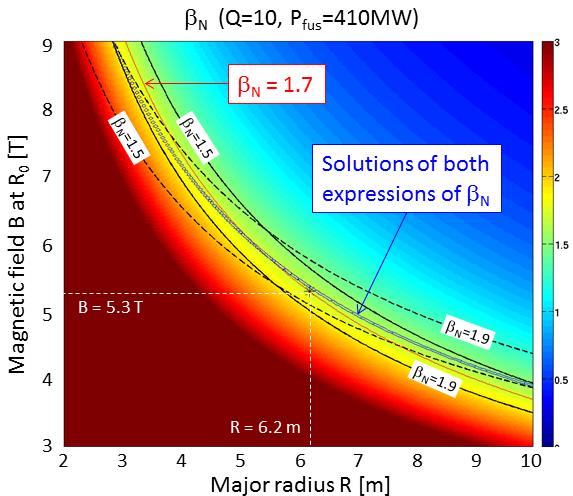
\includegraphics[width=0.75\textwidth]{figures/Fig_2D_betaN_R_B_ITER_ok.png}
		\caption{Map of $\beta_N=f(R,B)$ solutions of eq.\ref{eq:DT_fusion_power_betaN} and eq.\ref{eq:nTtau_betaN}.}
		\label{fig:solutions_betaN}
	\end{center}
\end{figure}

\begin{figure} 
	\begin{center}
		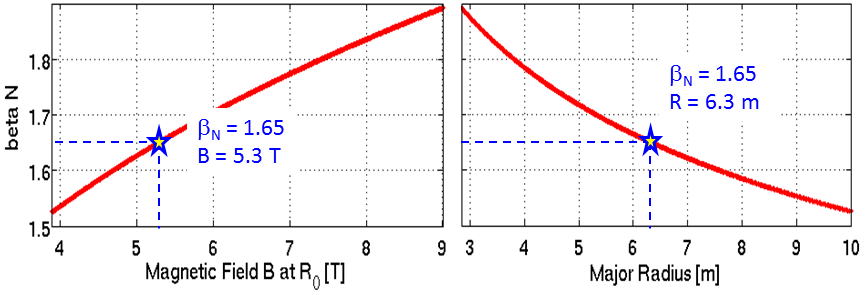
\includegraphics[width=1.\textwidth]{figures/Fig_betaN_solutions_2graphsRB.png}
		\caption{Solution values of $\beta_N$ (taken along the blue line of fig.\ref{fig:solutions_betaN}). The star is close to the ITER specifications in terms of $R$, $B$ and $\beta_N$.}
		\label{fig:}
	\end{center}
\end{figure}
